\documentclass{beamer}
\usepackage[utf8]{inputenc}
\usepackage[export]{adjustbox}
\usepackage{hyperref}
\hypersetup{
	colorlinks=true,
	urlcolor=adcorange,
	linkcolor=adcblue
}

\usetheme{Madrid}

\title{Multiplayer trivia game}
\subtitle{JavaScript and SocketIO part 1}
\author{Nathaniel Budijono}
\date{October 12, 2021}
\institute{UMN ADC}

\definecolor{adcblue}{RGB}{115,203,255}
\definecolor{adcorange}{RGB}{242,114,0}

\setbeamercolor{palette primary}{fg=white,bg=adcblue}
\setbeamercolor{palette secondary}{fg=adcorange,bg=white}
\setbeamercolor{structure}{fg=adcblue,bg=white}
\setbeamercolor{title in head/foot}{fg=adcblue,bg=white}
\setbeamercolor{date in head/foot}{fg=gray,bg=white}
\setbeamercolor{palette tertiary}{fg=white,bg=adcorange}

\begin{document}

\begin{frame}
    \titlepage
    \includegraphics[width=0.25\textwidth, right]{figs/ADC_Logo_Blue.png}
\end{frame}

\begin{frame}{Officer openings!}
	\begin{itemize}
		\item Workshop instructors
		\item Marketing director
	\end{itemize}

	\bigskip

	DM us on the discord!

	\bigskip

	\href{https://z.umn.edu/ADCdiscord}{https://z.umn.edu/ADCdiscord}
\end{frame}

\begin{frame}{A look ahead...}
	\centering
	{\Huge Guest Speaker Event: Postman API 101!}

	\bigskip

	November 2nd, 5-6pm

	\bigskip

	Tate Hall B20
\end{frame}

\begin{frame}{Follow the guide!}
	\centering
	\href{https://z.umn.edu/adc-mtg}{https://z.umn.edu/adc-mtg}

	\bigskip

	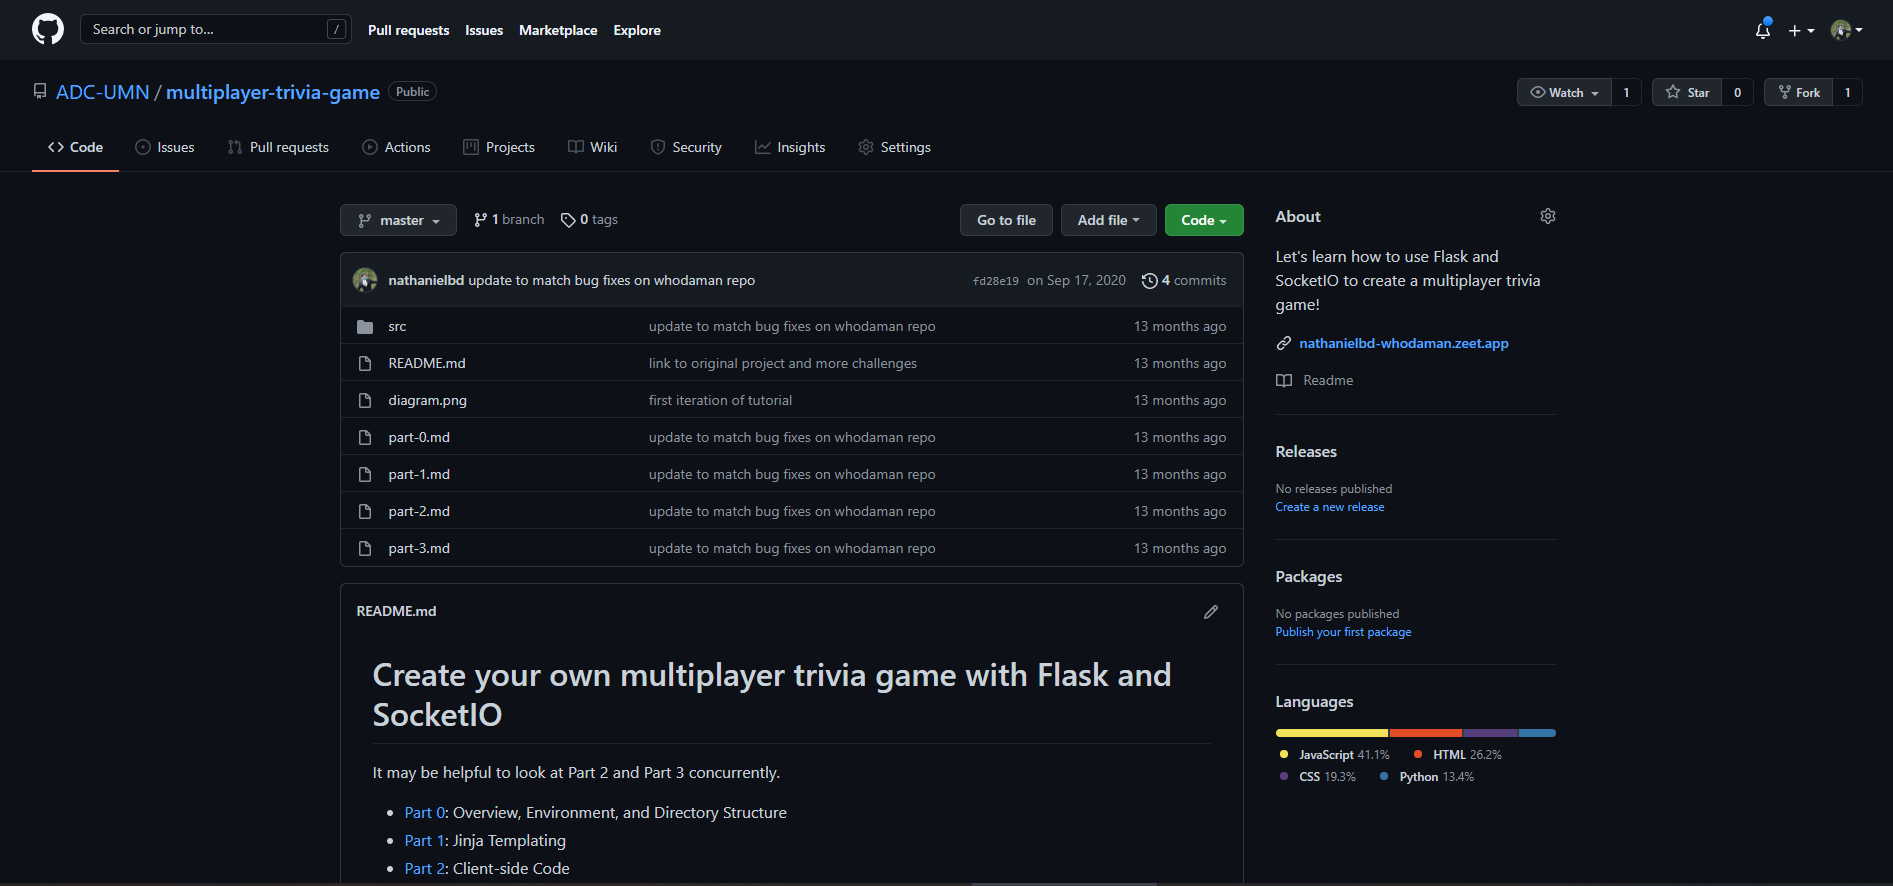
\includegraphics[width=0.9\textwidth]{figs/guide.png}
\end{frame}

\begin{frame}{The questions workflow}
	\only<1>{
	\begin{columns}
		\begin{column}{0.5\textwidth}
			Before


			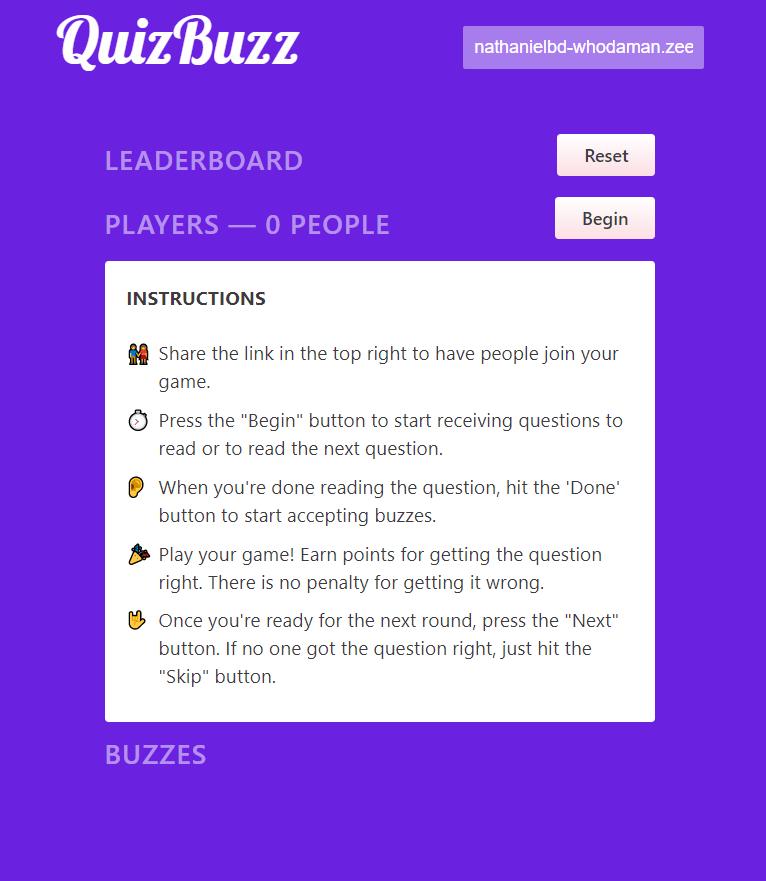
\includegraphics[width=0.9\textwidth]{figs/admin-landing.png}
		\end{column}

		\begin{column}{0.5\textwidth}
			After

			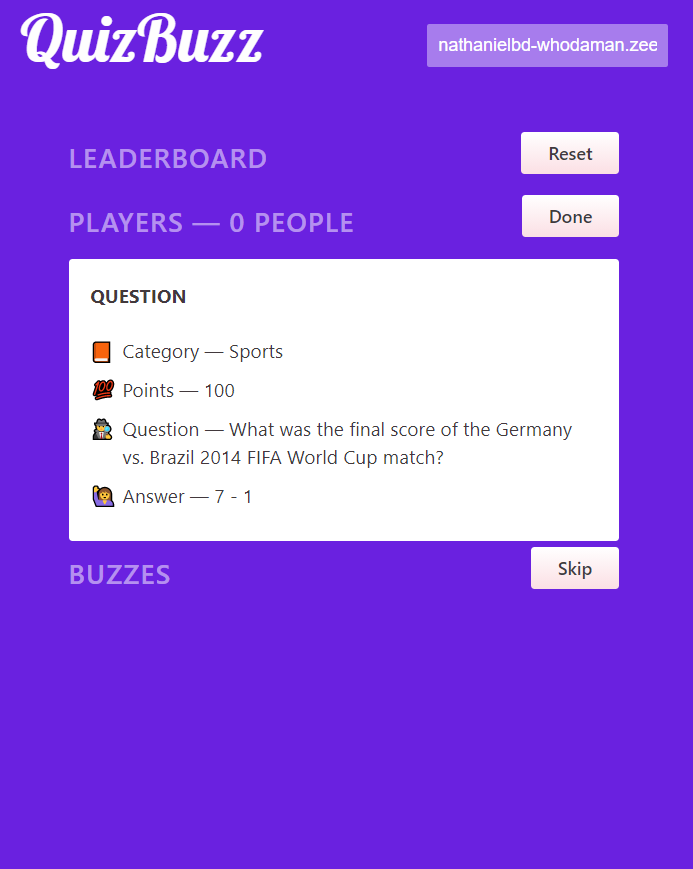
\includegraphics[width=0.9\textwidth]{figs/admin-question.png}
		\end{column}
	\end{columns}
	}
	\only<2>{
		\begin{center}
			\texttt{admin.js} \\
			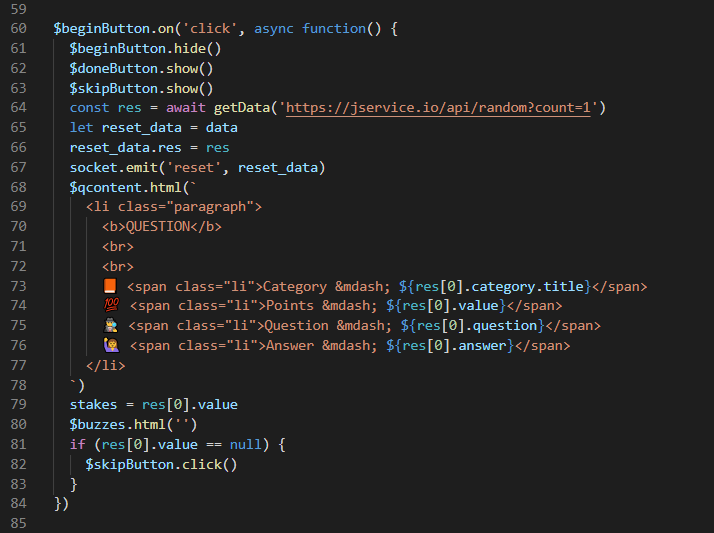
\includegraphics[width=0.8\textwidth]{figs/begin-button.png}	
		\end{center}
	}
	\only<3>{
		\begin{center}
			\texttt{app.py} \\
			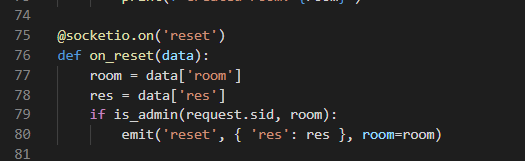
\includegraphics[width=0.8\textwidth]{figs/reset.png}
		\end{center}
	}
	\only<4>{
		\begin{center}
			\texttt{play.js} \\
			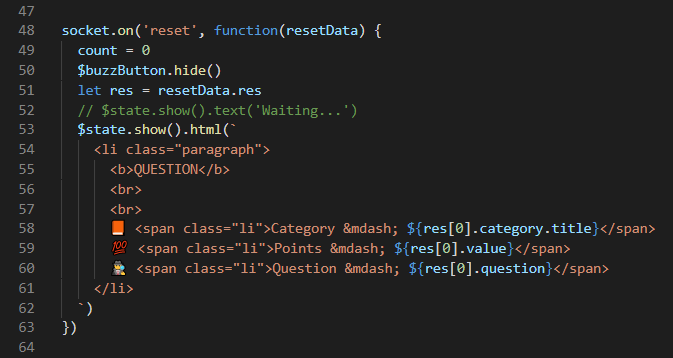
\includegraphics[width=0.9\textwidth]{figs/reset-play.png}
		\end{center}
	}
\end{frame}

\begin{frame}{Stuff to think about for features}
	Think about global variables needed in \texttt{app.py} or \texttt{<client>.js} \pause

	\bigskip

	\begin{enumerate}
		\item \texttt{<client>.js} emits an event, perhaps with data \pause
		\item \texttt{app.py} performs security checks and broadcasts the event \pause
		\item \texttt{<client>.js} listens for event, updates global variables, and updates the UI
	\end{enumerate}
\end{frame}

\begin{frame}{Futher reading}
	You can look at the guides for details on the other uses of SocketIO!

	\bigskip

	\href{https://github.com/ADC-UMN/multiplayer-trivia-game/blob/master/part-2.md}{https://github.com/ADC-UMN/multiplayer-trivia-game/blob/master/part-2.md}

	\bigskip

	\href{https://github.com/ADC-UMN/multiplayer-trivia-game/blob/master/part-3.md}{https://github.com/ADC-UMN/multiplayer-trivia-game/blob/master/part-3.md}
\end{frame}

\begin{frame}{A challenge}
	Try implementing new features!

	\pause

	\bigskip

	Fork \href{https://github.com/ADC-UMN/whodaman-ce}{https://github.com/ADC-UMN/whodaman-ce} to get started!

	\pause

	\bigskip

	Some ideas:
	\begin{itemize}
		\item Try implementing `Daily Doubles'! \pause
		\item Try implementing real-time chat for the players! \pause
		\item Add a feature to the landing page to display rooms in progress \pause
		\item Add a menu to the admin page to configure things like what types of questions are used, a timer/max number of questions system, or other settings!
	\end{itemize}
\end{frame}

\end{document}